\begin{Exc}{(A5.16.v0, 5 points):}
Consider an alternative validity condition for binary consensus: There must
be at least one admissible execution with decision value 0, and there
must be at least one admissible execution with decision value 1.
Show that there is no wait-free algorithm for this modified consensus
problem in single-writer shared memory asynchronous systems.
\end{Exc}

The solution to this exercise is almost identical to the case of a binary consensus algorithm
with unmodified validity. We present a modified proof for the existence of a bivalent initial
configuration, and then apply Lemma $255'$\footnote{Lemmas from the slides are
distinguished by appending the `prime' character to the lemma number.} directly. The modified
validity condition is referred to as alternative validity (AV) in the remainder of this exercise.

\begin{lemma}
Every wait-free binary consensus algorithm with the AV condition has a bivalent initial
configuration.
\end{lemma}

\begin{proof}
By contradiction, assume all initial configurations to be univalent. By AV, there must exist
at least one 0-valent, and at least one 1-valent initial configuration. In particular, there exist
a 0-valent initial configuration $I_0$ and a 1-valent initial configuration $I_1$ which differ
only in the input value of a single processor $p_i$\footnote{Begin at an initial configuration with all
inputs set to 0, and w.l.o.g. let that configuration be 0-valent. Then, iterate through all possible
initial configurations by toggling the inputs of processors one by one. Since a 1-valent initial
configuration exists by AV, at some point we must reach a configuration that is 0-valent, but toggling
of the input of a single processor produces a 1-valent configuration.}.

Let $\sigma$ be a schedule in which $p_i$ fails initially and all other processors are correct.
Since $I_0$ is 0-valent, all correct processors must eventually decide $0$ in $\alpha_0 = \sigma(I_0)$.
Applying the same schedule to $I_1$ results in an execution $\alpha_1 = \sigma(I_1)$ that is
$p_j$-similar to $\alpha_0$ for all $j \neq i$, and therefore must also decide $0$. This however
contradicts the 1-valence of $I_1$.
\end{proof}

The following lemma is identical to Lemma $255'$ from the lecture slides.
It is independent of the validity condition and thus may be applied here without modification.

\begin{lemma}
Every bivalent configuration of a wait-free binary consensus algorithm has at least one bivalent
successor configuration.
\end{lemma}

\begin{theorem}
There is no wait-free algorithm for the consensus problem in single-writer shared memory
asynchronous systems with the modified validity condition AV.
\end{theorem}

\begin{proof}
It follows directly from the preparation lemmas that there exists an execution in which
all configurations are bivalent, hence contradicting termination.
\end{proof}

% ------------------------------------------------------------------------------

\begin{Exc}{(L6.1.v0, 4 points):}
It is known that one can solve synchronous consensus
in the presence of $f=1$ Byzantine faulty processors
in a fully connected system of $n=4$ processors. Using an easy
impossibility proof, show that this is no longer possible when
two processors cannot communicate directly with each other.
\end{Exc}

\begin{theorem}
There is no algorithm that can solve synchronous consensus with $1$ Byzantine
processor in a system of $4$ processors which are not fully connected.
\end{theorem}

\begin{proof}
Consider a graph $G$ (Figure \ref{fig:g}) with nodes $\{p_0, p_1, p_2, p_3\}$, in which
node $p_0$ has no direct connection to node $p_3$. Assume that an algorithm $A$
exists (s.t. node $p_i$ locally executes algorithm $A_i$ for all $i$)
that solves synchronous consensus with at most one Byzantine processor in system $G$.

\begin{figure}[ht]
\centering
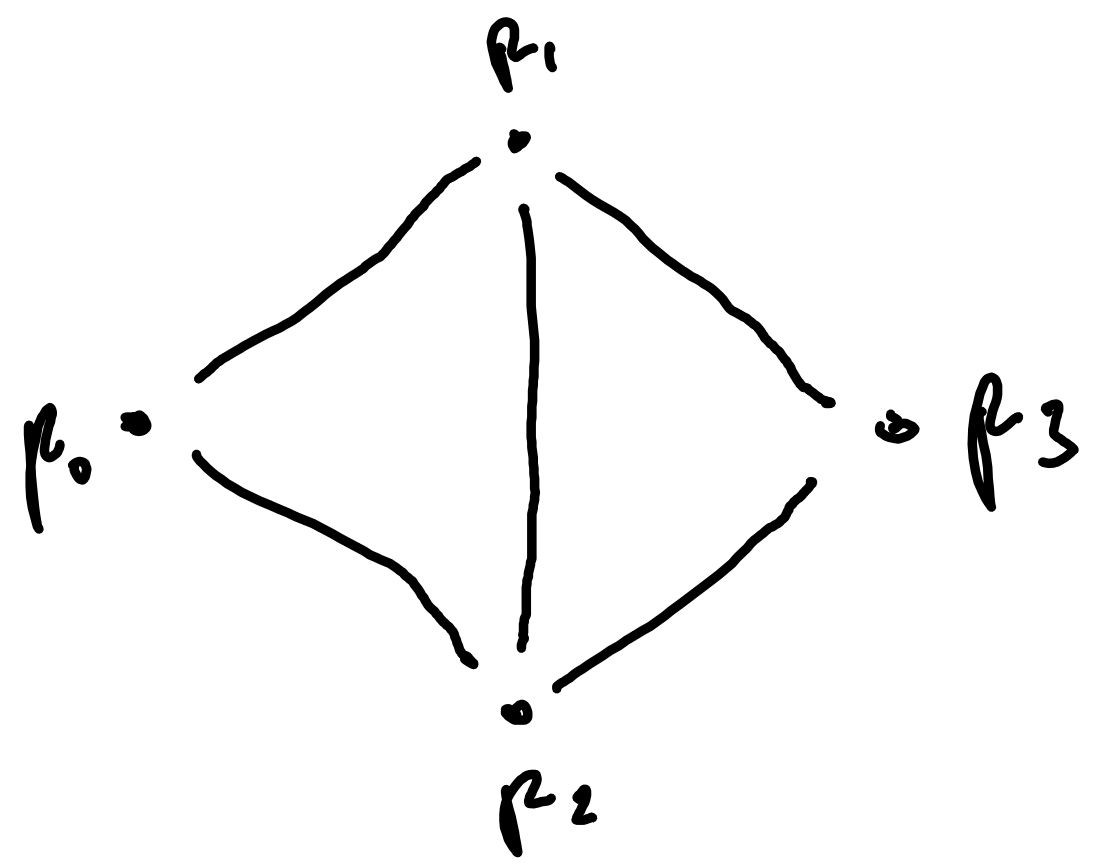
\includegraphics[width=0.5\textwidth]{fig_g}
\caption{The graph $G$. Nodes $p_0$ and $p_3$ are not connected.} \label{fig:g}
\end{figure}

Graph $G'$ (Figure \ref{fig:gprime}) is constructed in a way that is locally
indistinguishable from $G$ for each node. For all $i$, let nodes $p_i, p'_i$ execute $A_i$,
and let the input of nodes $\{p_0, p_1, p_2, p_3\}$ equal $0$ while the input of 
$\{p_0', p_1', p_2', p_3'\}$ equals $1$.

\begin{figure}[ht]
\centering
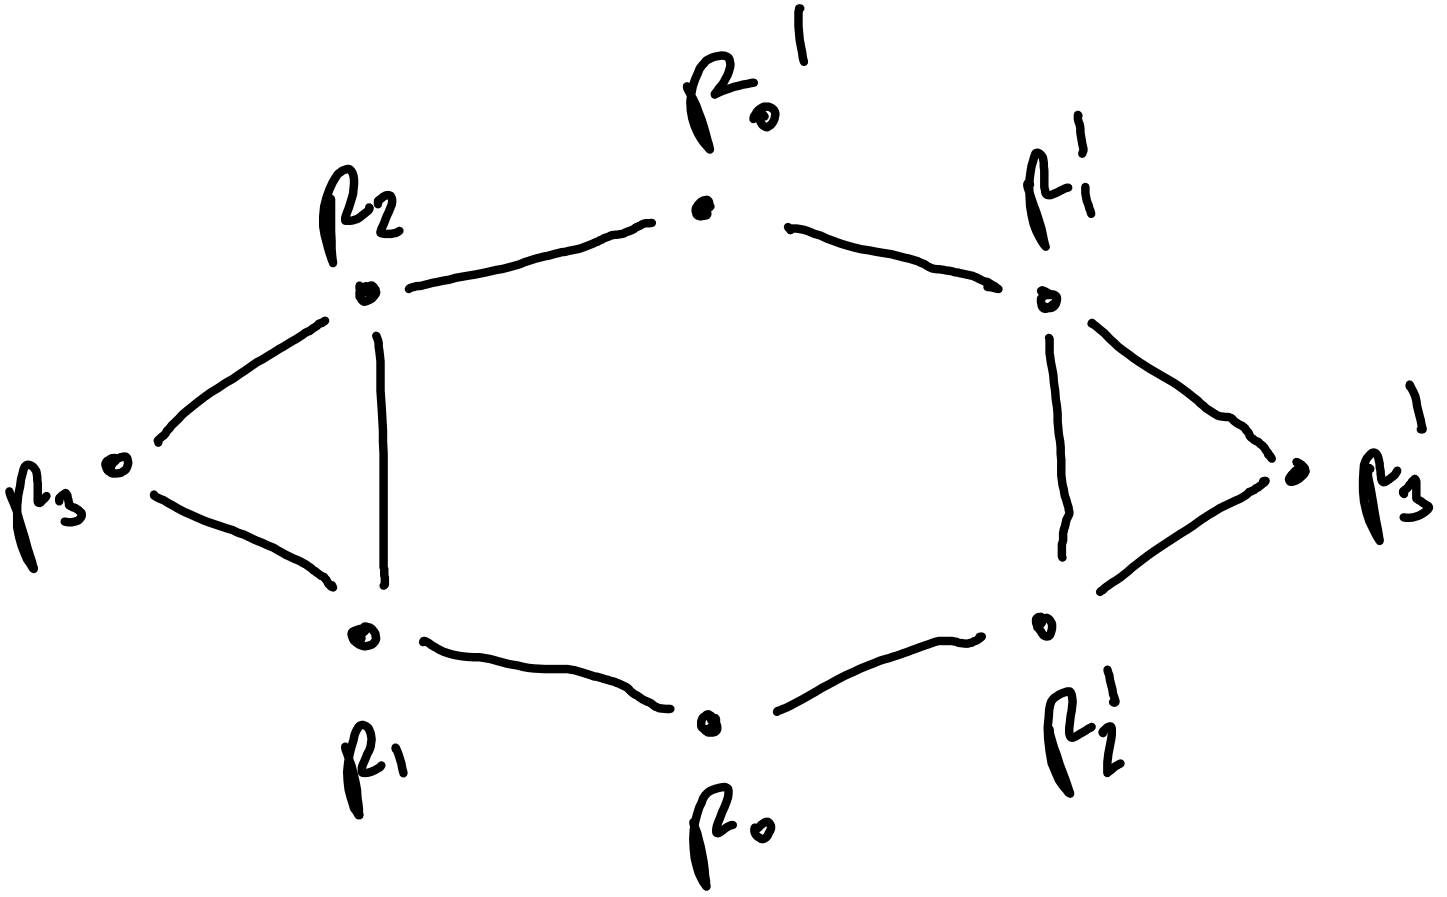
\includegraphics[width=0.5\textwidth]{fig_gprime}
\caption{The graph $G'$, locally indistinguishable from $G$.} \label{fig:gprime}
\end{figure}

Observe first the local subsystem $G'_0$ of $G'$ consisting of nodes $\{p_0, p_1, p_3\}$
plus the remaining edges to $\{p_2, p_2'\}$. This system equivalent to $G$ in which
node $p_2$ is faulty. By definition, $A$ can tolerate one Byzantine processor,
and by validity, all correct processors $\{p_0, p_1, p_3\}$ must decide $0$.

Similarly, the local subsystem $G'_1$ consisting of nodes $\{p_1', p_2', p_3'\}$
plus the remaining edges to $\{p_0, p_0'\}$ is equivalent to $G$ in which node
$p_0$ is faulty. Argumenting as above, nodes $\{p_1', p_2', p_3'\}$ must decide $1$.

Finally, observe the subsystem $G'_?$ consisting of nodes $\{p_0, p_2', p_3'\}$
plus the remaining edges to $\{p_1, p_1'\}$. Again, $G'_?$ is locally equivalent
to $G$ in which node $p_1$ is faulty. By agreement, all correct nodes must decide
$0$, or all correct processors must decide $1$.
However, we have previously established that processor $p_0$ decides $0$,
and processor $p'_2$ decides $1$, a contradiction.

Therefore no such algorithm $A$ can exist.
\end{proof}

% ------------------------------------------------------------------------------

\begin{Exc}{(S.5.4.v0, 7 points):}
Consider a lockstep synchronous system, where processors never fail but
messages can be lost arbitrarily. Prove that it is impossible to solve
binary consensus with the alternative validity property
\begin{itemize}
\item If all processors start with the same
input value, then every processor~$p_i$ computes
\begin{itemize}
%\itemsep-2pt
\item $y_i=1$ if $\forall j: x_j=1$ and no message got
lost in the entire execution,
\item $y_i=0$ if $\forall j: x_j=0$,
\end{itemize}
\end{itemize}
in a system of $n=2$ processors. Does this impossibility also
hold for the following variants of consensus:
\begin{enumerate}
\item[(a)] Ordinary consensus, i.e., agreement, termination and
the standard validity property from the textbook?
\item[(b)] Consensus with unanimous termination, i.e., agreement and
validity from the textbook, and the requirement that
\begin{itemize}
\item if some processor decides, all processors eventually decide, plus
\item if no message is lost, all processors eventually decide?
\end{itemize}
\end{enumerate}
\end{Exc}

\begin{lemma} \label{lemma:initial_univalent}
The initial configuration in a system of two processors $p_0, p_1$ with $x_0 = x_1 = 1$
is 1-valent.
\end{lemma}

\begin{proof}
Fix any algorithm $A$ and any schedule $\alpha$ in which no message is lost.
By the alternative validity (AV) condition, both processors must decide $1$
in $\alpha$, and by termination the algorithm must eventually terminate.

In the following, we show by bounded induction on the round number that all 
messages may be dropped without changing the decision of each
processor, and 1-valence follows for the initial configuration.

\emph{Induction base}: Consider the final round $r$ in $\alpha$; since all processors have
decided irrevocably, we can drop all messages in later rounds without changing the
outcome of the algorithm, and call this schedule $\alpha_{r+1}$.

\emph{Induction step}: Assume that we can drop all messages in rounds $\geq k + 1$ without
changing the eventual decision of each processor, and let that schedule be denoted $\alpha_{k+1}$.
Let $\alpha'_k$ be an
schedule identical to $\alpha_{k+1}$ except that all messages sent from $p_0$ to $p_1$ in round $k$
are dropped (if any exist). Since
$\alpha'_k \stackrel{p_0}{\sim} \alpha_{k+1}$, $p_0$ must still decide $1$, and agreement
forces $p_1$ to concur eventually.
Likewise, let $\alpha_k$ be identical to $\alpha'_k$ except that all messages from $p_1$ to $p_0$
are dropped. By similarity ($\alpha_k \stackrel{p_1}{\sim} \alpha'_k$) and agreement, the eventual
decision again remains unchanged; and since all messages in rounds $\geq k$ have been dropped, the
desired schedule has been found.
\end{proof}

% QUESTION: Semantics of dropping messages in a schedule <-> execution. Schedule is probably the
%           correct choice.
% QUESTION: 1-valency of initial state correct? I'm not sure... What if some specific subset of
%           messages is dropped?

\begin{theorem} \label{thm:no_av_consensus}
There is no binary consensus algorithm satisfying the alternative validity (AV)
condition for a system in which processors never crash but messages can be
lost arbitrarily,
\end{theorem}

\begin{proof}
By contradiction, assume such an algorithm $A$ exists.
Let $G^{ij}$ be the two-processor system with processors
$p_0, p_1$ such that $x_0 = i, x_1 = j$.

By Lemma \ref{lemma:initial_univalent} the initial configuration of
$G^{11}$ ($C^{11}$) is 1-valent; and by AV the initial configuration
of $G^{00}$ ($C^{00}$) is 0-valent.

Consider a system $G^{01}$ with initial state $C^{01}$.
Observe that $C^{00}$ is $p_0$-similar to $C^{01}$, $p_0$ must eventually decide 0.
Likewise, $C^{11}$ is $p_1$-similar to $C^{01}$; hence $p_1$ must eventually
decide 1, contradicting agreement.
\end{proof}

\begin{theorem}
There is no algorithm for ordinary binary consensus
for a system in which processors never crash but messages can be
lost arbitrarily,
\end{theorem}

\begin{proof}
The basic argument is the same as in the proof to Theorem \ref{thm:no_av_consensus},
but without requiring Lemma \ref{lemma:initial_univalent}. Definitions of
$G^{ij}$ are as in Theorem \ref{thm:no_av_consensus}.

By validity, the initial configuration of
$G^{11}$ ($C^{11}$) is 1-valent, and the initial configuration
of $G^{00}$ ($C^{00}$) is 0-valent.

Again, the initial state $C^{01}$ of $G^{01}$ is indistinguishable to $C^{00}$
($C^{11}$) for $p_0$ ($p_1$) and must therefore decide $0$ ($1$) in every extension
on $C^{01}$, contradicting agreement.
\end{proof}

\begin{theorem} \label{thm:no_at_consensus}
There is no algorithm for binary consensus satisfying the alternative termination (AT)
condition for a system in which processors never crash but messages can be
lost arbitrarily,
\end{theorem}

\begin{proof}
Definitions of
$G^{ij}$ are as in Theorem \ref{thm:no_av_consensus}.
Consider a system of two processors, and an arbitrary execution $\alpha$ in which
no messages are lost. By AT, all processors must eventually decide. By the same
argument as in Lemma \ref{lemma:initial_univalent}, all messages may be dropped
from $\alpha$ without changing the ultimate decision and the fact that all
processors eventually decide.

Thus an execution on $G^{11}$ ($G^{00}$) in which all messages are dropped must eventually 
decide $1$ ($0$).
Again, the initial state $C^{01}$ of $G^{01}$ is indistinguishable to $C^{00}$
($C^{11}$) for $p_0$ ($p_1$) and must therefore decide $0$ ($1$) in every extension
on $C^{01}$ in which all messages are dropped, contradicting agreement.
\end{proof}

% ------------------------------------------------------------------------------

\begin{Exc}{(S.5.14.v0, 6 points):}
Consider synchronous consensus with at most $f$ crash failures in not
fully connected communication graphs $G$.
\begin{enumerate}
\item[(1)] Using a partitioning argument, prove that there is no solution for this problem if $G$
is not $f+1$-connected.
\item[(2)] Extend the proof of the termination time lower bound of $f+1$ rounds
for fully connected communication graphs: Prove that every algorithm ${\cal A}$
(that may know $G$) for $n\geq f+2$ processors needs at least $f+Radius(G)$ rounds
for termination.

Research problem (optional): You may win extra points by either improving this
bound (I conjecture that the actual bound is $f+Diam(G)$) or else
by giving an algorithm and a proof that it indeed terminates in
$f+Radius(G)$.
\end{enumerate}
\end{Exc}

\begin{theorem}
There is no algorithm that can solve synchronous consensus with at most $f$
crash failures in a system $G$ that is less than $f+1$ connected.
\end{theorem}

\begin{proof}
Fix any system $G$ that is less than $f+1$ connected and any synchronous consensus
algorithm $A$. Divide $G$ into two components $G_0, G_1$ connected by at most $f$
edges (such a division must exist since $G$ is at most $f$-connected), and let
$E$ be the set of these edges.

Consider an execution of $A$ on this system in which the set of processors
$p_{faulty} = G_0 \cap E$ fail in the initial round, i.e. they never send
a message, and call the resulting schedule $\alpha$.
Note that $\alpha$ is admissible, since $|p_{faulty}| \leq f$.

Let $G^{ij}$ be an assignment of input values to $G$ such that all processors in $G_0$
have input $i$ while all in $G_1$ have input $j$.
Note that by validity, $\alpha(G^{00})$ must decide $0$ while $\alpha(G^{11})$ must decide $1$.

Consider the assignment $G^{01}$;
the components $G_0$ and $G_1$ are completely isolated and no messages are ever exchanged between
them. Since $\alpha(G^{01}) \stackrel{G_0}{\sim} \alpha(G^{00})$, all processors must decide
$0$. However, $\alpha(G^{01}) \stackrel{G_1}{\sim} \alpha(G^{11})$ implies that all processors
must decide $1$, a contradiction.
\end{proof}

For the lower bound proof, fix any algorithm $A$ solving synchronous consensus
while tolerating up to $f$ crash failures. $A$ is applied in a system $G$ of
$n \geq f+2$ processors that is at least $f+1$ connected.

\begin{lemma}
For each $k, 0 \leq k < f$, there is a $k$-round execution of $A$ that ends in
a bivalent configuration.
\end{lemma}

\begin{proof}
Equivalent to proof for Lemma 219' in the lecture slides.
\end{proof}

\begin{lemma} \label{lemma:indist_dist}
For any execution $\alpha$ ending after round $r$ in a system $G$: the failure-free
extension $\alpha'$ and the the extension $\alpha''$ in which $p_i$ fails in round $r+1$,
is indistinguishable to processors at distance $\geq k$ from $p_i$ until round $r+k$.
\end{lemma}

\begin{proof}
By induction on the distance $k$ from $p_i$. Let $P_k$, $P_{>k}$, and $P_{\geq k}$ denote,
respectively, the set of all processors at distance equal to, greater than, and
greater or equal to $k$ from $p_i$.

Induction base: By the definition of our model, the only difference 
between $\alpha'$ and $\alpha''$ in round $r+1$ is that $p_i$ potentially fails
to deliver messages to a subset of its neighbors $P_1$, and thus $\alpha'$ and $\alpha''$
are locally indistinguishable for all processors in $P_{>1}$ (if such processors exist).

Induction step: Assume that until round $r+k-1$, $\alpha'$ and $\alpha''$ are
indistinguishable to all processors in $P_{\geq k-1}$. In round $r+k-1$, processors
$P_{>k-1}$ receive messages only from processors in $P_{\geq k-1}$. These messages
originated in the computation step of round $r+k-2$, in which processors in $P_{\geq k-1}$
could not distinguish between $\alpha'$ and $\alpha''$ by assumption.
Therefore, processors in $P_{>k-1} = P_{\geq k}$ cannot distinguish between
$\alpha'$ and $\alpha''$ at least until round $r+k$.
\end{proof}

\begin{definition}
Let $G'_\alpha$ be the graph produced by removing all processors that fail
in execution $\alpha$ from the initial graph $G$.
\end{definition}

\begin{lemma}
If $\alpha_{f-1}$ is an $f-1$ round execution of $A$ that ends in a bivalent
configuration $C_{f-1}$, then there is a $Radius(G'_{\alpha_{f-1}})$ round extension 
in which some correct processor has not decided.
\end{lemma}

\begin{proof}
Similar to Lemma $223'$.
If there exists a 1-round extension which ends in a bivalent configuration $C_f$,
apply this lemma to $C_f$. Otherwise, if all 1-round extensions lead to univalent
configurations:

Without loss of generality, let the failure-free 1-round extension $\beta_f$
end in a 1-valent configuration $C^\beta_f$, and the 1-round extension $\gamma_f$ in which
$p_i$ crashes result in a 0-valent configuration $C^\gamma_f$.

By Lemma \ref{lemma:indist_dist}, the extensions $\beta'_f$ of $\beta_f$ and 
$\gamma'_f$ of $\gamma_f$ are indistinguishable to processors at distance $k$
from $p_i$ until round $f+k-1$, and no such processor can decide
until then.

By the definition of $G'_{\alpha_{f-1}}$, there must exist processors having at 
least distance $Radius(G'_{\alpha_{f-1}})$ from $p_i$. 
Hence $f+Radius(G'_{\alpha_{f-1}})-1$ is a lower bound for the number
of rounds of $A$\footnote{Note that we cannot argue based on $Radius(G)$ since
the removal of faulty nodes potentially reduces the radius.}.
\end{proof}

\section{Review Feedback}

In general, a constructive and thorough review.

In exercise 3, I did not alter the proof for Lemma \ref{lemma:initial_univalent},
since similarity was already explicit; maybe you were did not notice the 
different indices? The proof for Theorem \ref{thm:no_at_consensus} was redone.

The solution to exercise 4 now argues using similar executions.

Grade: 1
